\documentclass[11pt]{beamer}
\usepackage{verbatim}
\usepackage{amsmath}
\usepackage{amsthm}
\usepackage{graphics}
\usepackage{color}
\usepackage{stmaryrd}\usefonttheme[onlymath]{serif}

\title{Progess Report 1}
\date{\today}
\author{Xie Li}
\begin{document}
\maketitle

\begin{frame}\frametitle{Overview of the Progress}
\begin{itemize}
\item Survey of Tools: \textsc{CBMC}, \textsc{NuSMV} and \textsc{CPAChecker}

\item Reading paper: things related to separation logic.
\item Survey of Papers and Slides:
\begin{itemize}
\item Slides from \textsc{CBMC} site.
\item Alessandro Cimatti et al. Integrating BDD-based and SAT-based Symbolic Model Checking.
\item E. Clarke et al. Symbolic Model Checking.
\item \textsc{NuSMV} 2.5 Tutorial and other related slides.
\item Slides from \textsc{CPAChecker} site.
\item 
\end{itemize}
\item Usage of the Tools and brief introduction to Algorithms.
\end{itemize}

\end{frame}


\begin{frame}\frametitle{Tool Survey: \textsc{CBMC}}
\textsc{CBMC} is a bounded model checker for C and C++.
\textbf{Functionalities:}
\begin{center}
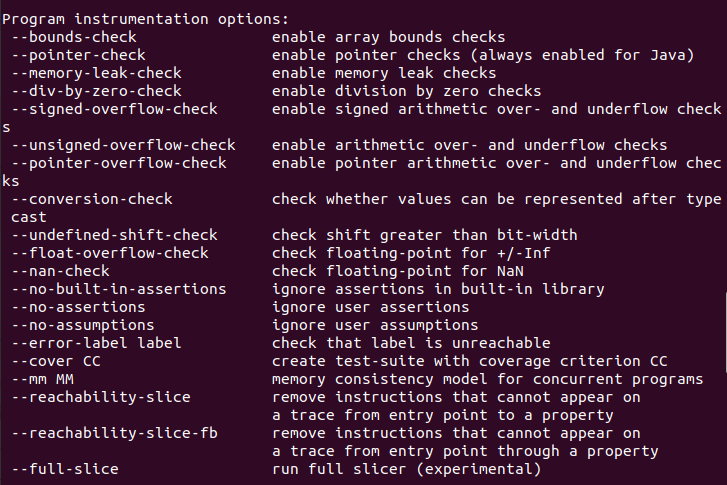
\includegraphics[scale=0.38]{funcCbmc.png}
\end{center}
\textbf{Usage:}
\texttt{cbmc input.c --bounds-check --pointer-check}
\end{frame}
\begin{frame}\frametitle{Insight of Algorithm}
\begin{center}
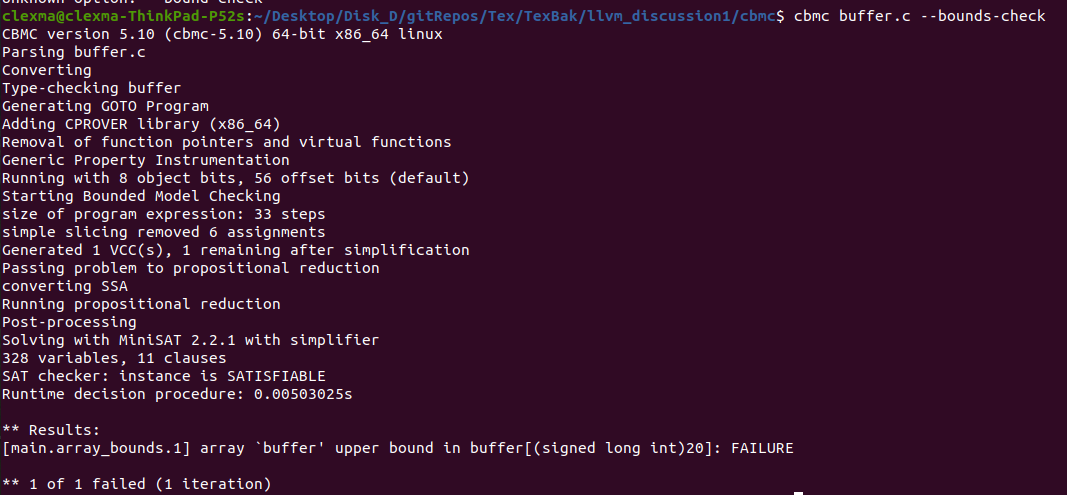
\includegraphics[scale=0.35]{expCbmc.png}
\end{center}
Slides from the official website of \textsc{CBMC}.
\end{frame}


\begin{frame}\frametitle{Tool Survey: \textsc{NuSMV}}
\textsc{NuSVM} is a NEW tool of Symbolic model checker for finite state systems.

\textbf{Features:}
\begin{itemize}
\item Analysis of invariants.
\item LTL model checking.
\item PSL model checking.
\item SAT-based bounded model checking.
\end{itemize}
The tool is given a SMV language file as input and 
\end{frame}

\begin{frame}\frametitle{Overview of \textsc{NuSMV}}
\begin{center}
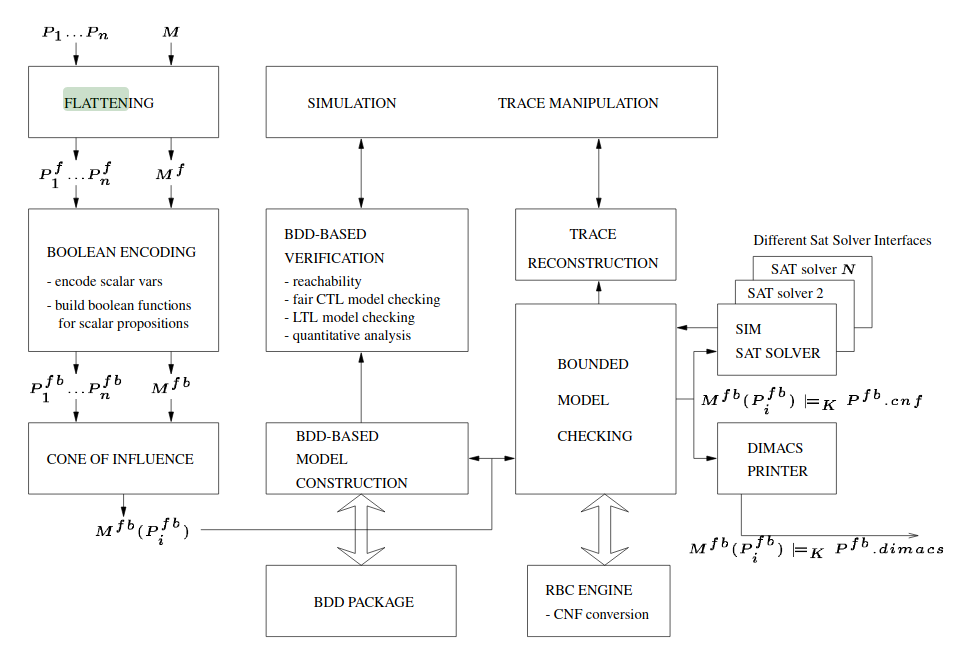
\includegraphics[scale=0.35]{nusmv_overview .png}
\end{center}
\end{frame}

\begin{frame}\frametitle{Input Format of \textsc{NuSMV}}

\begin{center}
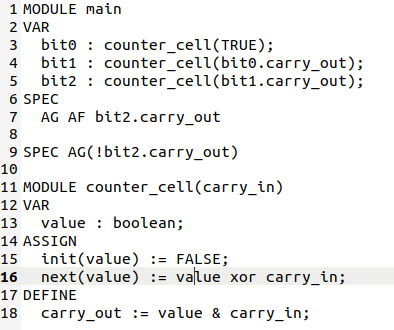
\includegraphics[scale=0.4]{nusmv_format.png}
\end{center}
\texttt{./NuSMV couter.smv}



\begin{center}
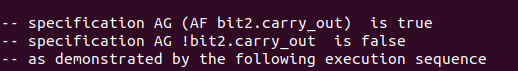
\includegraphics[scale=0.4]{nusmv_run.png}

\end{center}


\end{frame}


\begin{frame}\frametitle{Tool Survey: \textsc{CPAChecker}}
\textsc{CPAChecker} is a configurable software-verification platform that enables the parsing, analysing and verifying of the source program.

\begin{itemize}
\item Static Analysize: Data-Flow analysis etc.
\item Invariant generation via over-approximation.
\item Termination checking.
\item ...
\end{itemize}

\end{frame}
\begin{frame}\frametitle{Architecture}


\begin{center}
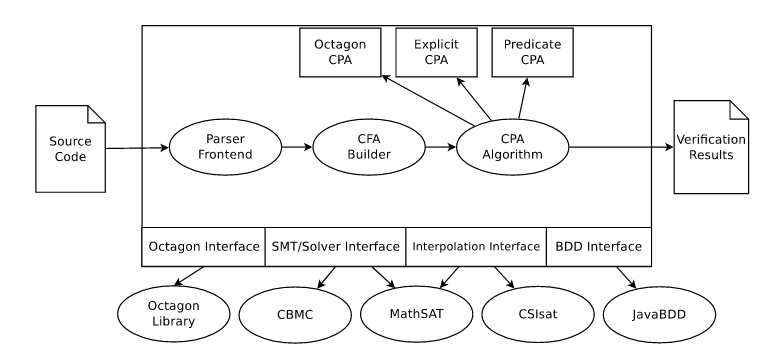
\includegraphics[scale=0.4]{cpa_arch.png}
\end{center}
\end{frame}


\begin{frame}\frametitle{Future Work}
\begin{itemize}
\item A closer look into the source code of these tools especially \textsc{CPAChecker}.

\item Better understanding of the underlying algorithm and techniques.

\item Other tool survey: \textsc{SPIN}, \textsc{Infer}, \textsc{KLEE}, etc.
\end{itemize}
\end{frame}
\end{document}